\documentclass[border=3mm]{standalone}

% Tikz related libraries. Primarily used for drawing small figures.
\usepackage{calc}
\usepackage{tikz}
\usetikzlibrary{matrix}
\usetikzlibrary{shapes,chains}

\tikzset{
  block/.style = {draw, fill=white, rectangle, minimum height=3em, minimum width=4em},
  input/.style = {coordinate},
  output/.style= {coordinate},
}

\begin{document}

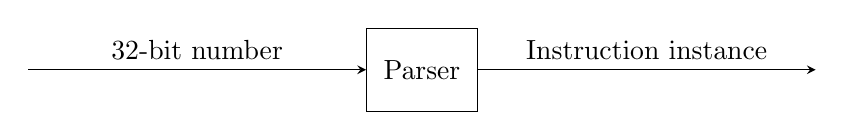
\begin{tikzpicture}[>=stealth, auto, node distance=5cm]
    \node [input] (input) {};
    \node [block, right of=input] (parser) {Parser};
    \node [output, right of=parser] (output) {};
    \draw [->] (input) -- node{32-bit number} (parser);
    \draw [->] (parser) -- node{Instruction instance}(output);
\end{tikzpicture}

\end{document}

